%%%%%%%%%%%%%%%%%%%%%%%%%% ch2 %概率论回顾全集备份
\begin{frame}
  \frametitle{主要内容}
  \tableofcontents[hideallsubsections]
\end{frame}

\section{随机变量}

\begin{frame}
随机事件的特征是不确定性,但是我们可以通过重复观测,从不确定现象中寻找、观察特定事件发生的规律,为此需要让某一随机现象重复发生(不一定是人为控制的)并记录观测结果,称之为随机试验。

随机试验的三个特征:
\begin{itemize}
	\item 可以在相同条件下重复进行;
	\item 试验的所有可能结果是明确可知的,并且不止一个;
	\item 每次试验总是恰好出现这些可能结果中的一个,但在一次试验之前却不能肯定这次试验会出现哪个结果。
\end{itemize}

\end{frame}

\begin{frame}{概率论中的三个组成部分}
\begin{itemize}
	\item 样本空间$\Omega$
	\item 事件域$\mathcal{F}$
	\item 概率$P$
\end{itemize}
\end{frame}


\begin{frame}
\begin{itemize}
	\item 样本空间$\Omega$:一个随机试验所有可能出现的结果的全体,称为随机事件的样本空间。\\
	每一个可能的结果称为基本事件,它们的全体就是样本空间。
	\item 样本点$\xi_k$:随机试验的一个结果,就是某个基本事件,也就是$\Omega$中的一个元素。\\
	$\Omega=\{\xi_k|k=1,\dots,n\}$
	\item 随机事件$A$: 样本空间中的某个子集称为随机事件,简称事件(事件是集合)。
    \item 事件域$\mathcal{F}$: 样本空间中的某些子集构成的满足如下条件的集合,称为事件域(又称$\sigma^-$域)。
	\begin{itemize}
		\item[(1)] $\Omega\in\mathcal{F}$
		\item[(2)] 若$A\in\mathcal{F}$, 则$A$的补$\overline{A}\in\mathcal{F}$
		\item[(3)] 若$A_n\in\mathcal{F}, n=1,2,\dots$, 则$\bigcap\limits_{n=1}^{\infty}A_n\in\mathcal{F}$
	\end{itemize}
\end{itemize}
\end{frame}

\begin{frame}
\begin{example}
	一个盒子中有10个相同的球,5各白色,5个黑色,搅匀后从中任意摸取一球。\\
	$\xi_1=\{\text{取得白球} \}$, $\xi_2=\{\text{取得黑球} \}$\\
	$\Omega=\{\xi_1,\xi_2\}$
\end{example}
\begin{example}
	一个盒子中有10个相同的球,编号1,2,...,10, 从中取一球。\\
	$\Omega=\{1,2,\dots,10\}$\\
	$A=\{\text{6号球} \}=\{6\}$, $B=\{\text{偶数编号球} \}=\{2,4,6,8,10\}$, $\overline{B}=\{\text{奇数编号球}\}$,$C=\{\text{编号小于等于5的球} \}=\{1,2,3,4,5\}$\\
	事件A是基本事件,而B和C则由多个基本事件所组成,并且$A,B,C\subset\Omega$。
\end{example}
\textit{空集$\emptyset$可以看作$\Omega$的子集,在任意一次试验中不可能有此事件发生,称为不可能事件。}
\end{frame}

\begin{frame}{事件$A$的概率$P(A)$}
  事件域中的元素就是随机事件。如果这些事件的随机性能够由定义在$\mathcal{F}$上的具有非负性,归一性和可列加性的实函数$P(A)$来确定,则称$P$是定义在二元组$(\Omega,\mathcal{F})$上的概率,而称$P(A)$为事件$A$的概率。
  \begin{enumerate}
  	\item[(1)] 非负性。 $P(A)\ge 0$
  	\item[(2)] 归一性。 $P(\Omega)=1$
    \item[(3)] 可列加性。$A_1,A_2,...,A_n$互不相容$(A_i\cap A_j=\emptyset,i\ne j)$,则$P(A_1\cup A_2\cup\dots\cup A_n) = P(A_1)+P(A_2)+\cdots+P(A_n)$
  \end{enumerate}
\end{frame}

\begin{frame}
	非空的事件域$\mathcal{F}$关于交、并、补、差元素是封闭的。
	\begin{enumerate}
		\item 若$A\in\mathcal{F}$, 则$\overline{A}\in\mathcal{F}$
		\item 若$A\in\mathcal{F},B\in\mathcal{F}$, 则$A\cup B\in \mathcal{F}$
		\item 若$A\in\mathcal{F},B\in\mathcal{F}$, 则$A\cap B\in \mathcal{F}$
		\item 若$A\in\mathcal{F},B\in\mathcal{F}$, 则$A- B\in \mathcal{F}$
	\end{enumerate}
	\begin{proof}
		由于$\mathcal{F}$为非空子集类,则若$A\in\mathcal{F}$,由(1)知,$\overline{A}\in\mathcal{F}$,又由(2)知$A\cup\overline{A}=\Omega\in\mathcal{F}$. 故有$\Omega\in\mathcal{F}$. \\
		若$A\in\mathcal{F},B\in\mathcal{F}$, 则$\overline{A}\in\mathcal{F}$, $\overline{B}\in\mathcal{F}$,那么$\overline{A}\cup\overline{B}\in\mathcal{F}$, 即有$A\cap B=\overline{\overline{A}\cup\overline{B}}\in\mathcal{F}$,故$\mathcal{F}$对交也封闭。\\
		再若$A,B\in\mathcal{F}$, 则有$A-B=A\overline{B}\in\mathcal{F}$, 即$\mathcal{F}$对交也封闭。\\
		由数学归纳法可证,若$A_i\in\mathcal{F}$, 则$\bigcup_{i=1}^{n}\in\mathcal{F}$
	\end{proof}
\end{frame}

\begin{frame}
\frametitle{古典概型}
\begin{itemize}
	\item 样本空间的元素(即基本事件)只有有限个,不妨设为$n$个,$\Omega=\{\xi_1,\xi_2,\dots,\xi_n\}$
	\item 每个基本事件出现的可能性是相等的,即有$P(\xi_1)=P(\xi_2)=\cdots=P(\xi_n)$
	\item 事件域$\mathcal{F}$为$\Omega$的所有子集的全体,即是$Pwr(\Omega),\Omega$的m幂集,共有$2^n$个事件,$\emptyset\in\mathcal{F},\Omega\in\mathcal{F}$。
	\item 由概率的有限可加性知\\
	$1=P(\Omega)=\Sigma_{i=1}^{n}P(\xi_i)\implies P(\xi_i)=\frac{1}{n},(i=1,\dots,n)$
	\item 对任意一个随机事件$A\subseteq\mathcal{F}$, 如果$A$是$k$个基本事件的和,即$A=\{\xi_{i_1}\}\cup \{\xi_{i_2}\}\cup\cdots\cup\{\xi_{i_k}\}$, 则
	$$P(A)=\frac{k}{n}=\frac{\text{$A$中所包含的基本事件数}}{\text{基本事件总数}}$$
\end{itemize}
\end{frame}

\begin{frame}
\frametitle{样本空间的选取}
为求一个事件的概率,样本空间可以有不同的取法,但一定要认真,基本事件和求概事件数的计算都要在同一个样本空间中进行,否则会导致谬误!
\begin{example}
	一个盒子中有10个相同的球,编号1,2,...,10, 从中取一球,求此球的号码为偶数的概率。\\
	$\Omega=\{1,2,\dots,10\}$\\
	$A=\{\text{偶数编号球} \}=\{2\}\cup\{4\}\cup\{6\}\cup\{8\}\cup\{10\}=\{2,4,6,8,10\}$。\\
	$P(A)=\frac{|A|}{n}=\frac{5}{10}=\frac{1}{2}$
\end{example}
另外一种解法:$\Omega=\{A,\overline{A}\},A=\{\text{编号为偶数的球}\},\overline{A}=\{\text{编号为奇数的球}\},\mathcal{F}=\{\emptyset,\Omega,A,\overline{A}\}$,由$A,\overline{A}$的对称性,即得$P(A)=\frac{1}{2}$

\end{frame}

\begin{frame}
\frametitle{样本空间的选取}
\begin{block}{Notes}
	两种解法的样本空间$\Omega$不同(从而事件域$\mathcal{F}$是不同的)。严格地说,两者所描述的随机试验是不同的。例如对于第二种解法来说,$B=\{\text{号码为4的球}\}$并不属于事件域$\mathcal{F}$,就是说$B$不是一个事件,从而也就没有概率可言。但对第一种解法,$B$是事件,而且$P(B)=\frac{1}{10}$。
\end{block}

\end{frame}

\begin{frame}
\begin{example}
	甲、乙两人掷硬币,其中甲掷$n+1$次,乙掷$n$次。求``甲掷出正面的次数大于乙掷出正面的次数"这一事件的概率。\\
	令\\ $A_1=$甲掷出正面的次数,$A_2=$甲掷出反面的次数,$B_1=$乙掷出正面的次数,$B_2=$乙掷出反面的次数。\\
	$\Omega-\{A_1 > B_1\}=\{A_2\le B_1\}=\{A_2>B_2\}$\\
	由对称性知\\
	$P(A_1>B_1)=P(A_2>B_2)$\\
	由此即得\\
	$P(A_1>B_1)=\frac{1}{2}$
\end{example}
\begin{block}{Notes}
	在古典概型中,所谓``等可能性'',正是``对称性"产生的结果,因为各个基本事件处在``对称"的位置上,所以才有``等可能性"。
\end{block}
\end{frame}

\begin{frame}{几何概率}
我们在一个面积为$S_\Omega$的区域$\Omega$中,等可能地任意投点,如果点落入小区域$S_A$中的可能性与$S_A$成正比,而与$A$的位置及形状无关。如果``点落入小区域$A$"这个随机事件仍然记为$A$,则由$P(\Omega)=1$可得
$$P(A)=\frac{S_A}{S_\Omega}$$
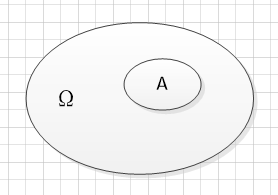
\includegraphics[scale=0.4]{geometry}
\end{frame}

\begin{frame}
\begin{example}
	(会面问题)甲、乙两人约定在6时到7时之间在某处会面,并约定先到者应等候另一个人一刻钟,过时即可离去。求两人能会面的概率。\\
	如图,以x,y表示甲乙两人,则两人能会面的充要条件是: $|x-y|\leq 15$\\
	$$P(A)=\frac{S_A}{S_\Omega}=\frac{60^2-45^2}{60^2}=\frac{7}{16}$$
	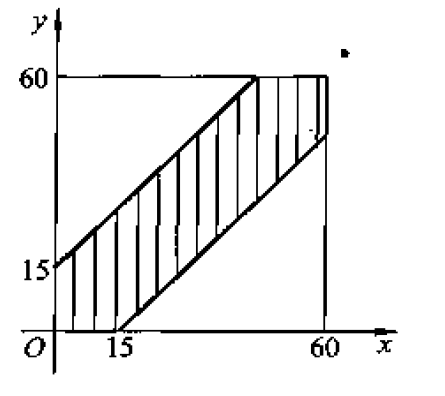
\includegraphics[scale=0.4]{geometry1}
\end{example}
\end{frame}

\section{条件概率}

\begin{frame}{概率的加法公式与条件概率}
如果有两个随机事件$A,B\in\mathcal{F}$,有如下加法公式:
\[P(A\cup B)=P(A)+P(B)-P(AB)\]
特备地,当$A,B$是补不相容的两个事件, 即$A\cap B=\emptyset$时, 有
\[P(A\cup B)=P(A)+P(B)\]

\begin{columns}
	\column{0.4\textwidth}%<1->
	\[P(A|B)=\frac{S_{AB}}{S_B}=\frac{S_{AB}/S_\omega}{S_B/S_\omega}=\frac{P(AB)}{P(B)} \]
	\column{0.4\textwidth}%<1->
	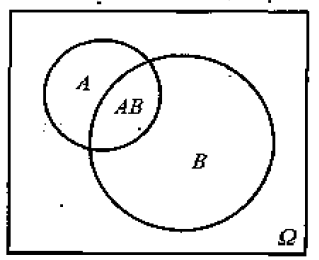
\includegraphics[scale=0.2]{P(AB)}
\end{columns}
\end{frame}

\begin{frame}{条件概率}
\begin{definition}
	若$\Omega,\mathcal{F},P$是一个概率空间,$B\in\mathcal{F}$, 且$P(B)>0$,则对任意的$A\in\mathcal{F}$,称
	$$P(A|B)=\frac{P(AB)}{P(B)}$$
	为在已知事件B发生的条件下,事件A发生的条件概率。
\end{definition}

\begin{columns}%0.6 0.4表示相对比例
	\column{0.4\textwidth}%<1->
\[P(A|B)=\frac{S_{AB}}{S_B}=\frac{S_{AB}/S_\omega}{S_B/S_\omega}=\frac{P(AB)}{P(B)} \]
	\column{0.4\textwidth}%<1->
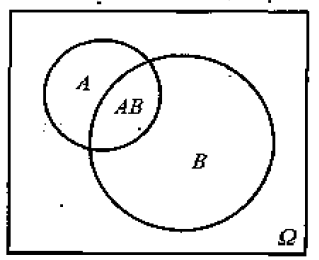
\includegraphics[scale=0.2]{P(AB)}
\end{columns}
\end{frame}

\begin{frame}{条件概率的性质及其推论}
\begin{block}{条件概率$P(\bullet|B)$的具备概率的三个基本性质}
	\begin{enumerate}
		\item 非负性: 对任意的$A\in F, P(A|B)\ge 0$;
		\item 规范性: $P(\Omega|B)=1$;
		\item 可列加性: 对任意的一列两两互不相容的事件$A_i(i=1,2,\dots)$, 有
		\[P\left[\bigcup\limits_{i=1}^{+\infty}(A_i|B)\right]=\sum\limits_{i=1}^{+\infty}P(A_i|B) \]
	\end{enumerate}
\end{block}
\begin{corollary}
概率的乘法公式:  $P(AB)=P(B)P(A|B)$
\end{corollary}

\begin{corollary}
	$P(A_1A_2\cdots A_n)=P(A_1)P(A_2|A_1)P(A_3|A_1A_2)\cdots P(A_n|A_1A_2\cdots A_{n-1})$
\end{corollary}
\end{frame}

\begin{frame}
\begin{example}
	一个家庭中有两个小孩,已知其中有一个是女孩,问这时另一个小孩也是女孩的概率有多大?\\
	$\Omega=$\{(男,男),(男,女),(女,男),(女,女)\}\\
	$A=$\{已知有一个是女孩\}=\{(男,女),(女,男),(女,女)\}\\
	$B=$\{另一个也是女孩\}=\{(女,女)\}\\
	于是所求概率为\\
	$P(B|A)=\frac{P(AB)}{P(A)}=\frac{1/4}{3/4}=\frac{1}{3}$
\end{example}
\end{frame}

\begin{frame}
差事件、条件事件或由差事件及条件事件复合而成的事件的概率均可化为$P(A),P(B),P(AB)$的形式。
例如
\[P(\overline{A\cup B})=1-P(A\overline{B})=1-[P(A)-P(AB)]=1-P(A)+P(AB) \]
\[P(A|\overline{B})=\frac{P(A)-P(AB)}{1-P(B)} \]
\begin{example}
	有外形相同的球分装在三个盒子,每盒10个。其中第一个盒子中7个球标有字母A,3个球标有字母B; 第二个盒子中有红球和白球各5个; 第三个盒子中则有红球8个,白球2个。试验按如下规则进行: 先在第一个盒子中任取一个球,若取得标有字母A的球,则在第二个盒子中任取一个球; 若第一次取得标有字母B的球,则在第三个盒子中任取一个球。如果第二次取出的是红球,则称试验成功。求试验成功的概率。
\end{example}
\end{frame}

\begin{frame}
\begin{solution}
	令$A=$\{从第一个盒子取得标有字母A的球\},$B=$\{从第一个盒子取得标有字母B的球\},$R=$\{第二次取出的球是红球\},$W=$\{第二次取出的球是白球\}。\\
	则容易球得: $P(A)=\frac{7}{10}, P(B)=\frac{3}{10}, P(R|A)=\frac{1}{2},P(W|A)=\frac{1}{2},P(R|B)=\frac{4}{5},P(W|B)=\frac{1}{5}$\\
	于是,试验成功的概率为
	\begin{align*}
	P(R)=P(R\cap\Omega)&=P[R\cap(A\cup B)]\\
	&=P(RA\cup RB)=P(RA)+P(RB)\\
	&=P(R|A)\cdot P(A)+P(R|B)\cdot P(B)\\
	&=\frac{1}{2}\cdot\frac{7}{10}+\frac{4}{5}\cdot\frac{3}{10}=0.59
	\end{align*}
	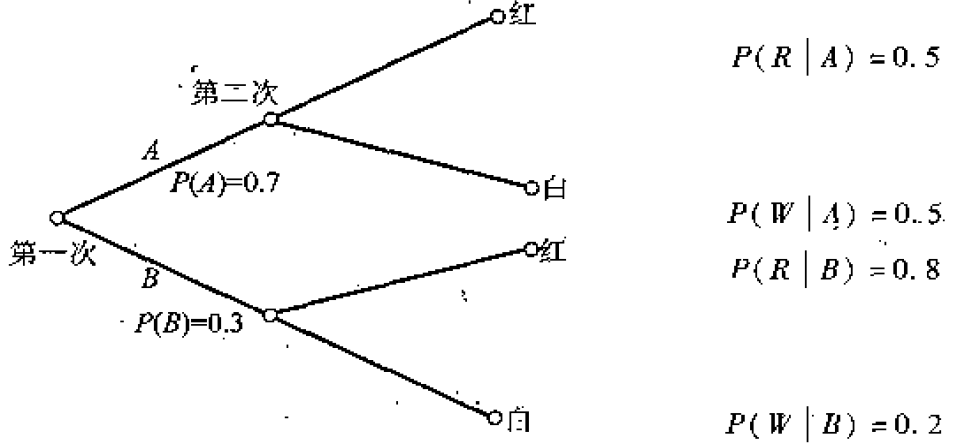
\includegraphics[scale=0.18]{tree}
\end{solution}
\end{frame}

\begin{frame}{概率树/全概率公式}
概率树思想:为了求解复杂事件的概率,往往可以先把它分解成两个(或若干个)互不相容的较简单的事件之并。求出这些较简单事件的概率,在利用加法公式即得所要求的复杂事件的概率。把这个方法一般化,便的到下述定理。
\begin{theorem}
	设$B_1,B_2,\cdots$是一列互不相容的事件,且有
	\[\bigcup_{i=1}^{+\infty}B_i=\Omega,P(B_i)>0 \]
	则对任一事件A,有
	\[P(A)=\sum_{i=1}^{+\infty}P(B_i)P(A|B_i) \]	
\end{theorem}
\end{frame}

\begin{frame}{概率树/全概率公式}
\begin{proof}
	\begin{align*}
	P(A)&=P(A\cap\Omega)=P[A\cap(\bigcup_{i=1}^{+\infty}B_i)]\\
	&=P[\bigcup_{i=1}^{+\infty}(AB_i)]=\sum_{i=1}^{+\infty}P(AB_i)\\
	&=\sum_{i=1}^{+\infty}P(B_i)P(A|B_i)
	\end{align*}
\end{proof}
\end{frame}

\begin{frame}
\begin{example}
	某工厂有4条流水线生产同一种产品, 该4条流水线的产品分别占总产量的15\%, 20\%, 30\%, 35\%, 又这4条流水线的不合格品率依次为0.05, 0.04, 0.03及0.02. 现从出厂产品中任取一件, 问(1) 恰好抽到不合格品的概率为多少? (2) 第4条流水线应承担的责任?
\end{example}
\end{frame}

\begin{frame}[shrink]
解: (1) 令
\begin{align*}
A&=\{\text{任取一件,恰好抽到不合格品} \}\\
B&=\{\text{任取一件,恰好抽到第$i$条流水线的产品}, (i=1,2,3,4) \}
\end{align*}
于是由全概率公式可得
\begin{align*}
P(A)&=\sum\limits_{i=1}^4P(B_i)P(A|B_i)=0.15\times 0.05+0.20\times 0.04+0.30\times 0.03+0.35\times 0.02\\
&=0.0315=3.15\%
\end{align*}
实际上,$P(A|B_i)$可以从过去生产的产品中统计出来,称为先验概率。\\
(2) 从概率论的角度考虑可以按$P(B_i|A)$的大小来追究第$i$条$i=1,2,3,4$流水线的责任。\\
$P(AB_4)=P(B_4)P(A|B_4)=0.35\times 0.02=0.007$\\
由条件概率的定义知
\begin{align*}
P(B_4|A)=\frac{P(AB_4)}{P(A)}=\frac{P(B_4)P(A|B_4)}{\sum\limits_{i=1}^4P(B_i)P(A|B_i)}=\frac{0.007}{0.0315}\approx=0.222
\end{align*}
\end{frame}

\begin{frame}{贝叶斯(Bayes)公式}
\begin{theorem}
	若$B_1, B_2, \dots$为一系列互不相容的事件, 且
	\[\bigcup\limits_{i=1}^{+\infty}B_i=\Omega \]
	\[P(B_i)>0, i=1,2,\dots \]
	则对任一事件A, 有
	\[P(B_i|A)=\frac{P(B_i)P(A|B_i)}{P(A)}=\frac{P(B_i)P(A|B_i)}{\sum\limits_{j=1}^{+\infty}P(B_j)P(A|B_j)}, \quad i=1,2,\dots \]
\end{theorem}
$P(B_i)$是试验以前就已经知道的概率---\textbf{先验(先于试验)概率}。\\
条件概率$P(B_i|A)$反映了试验以后,对A发生的``来源''的各种可能性的大小---\textbf{后验概率}。
\end{frame}

\begin{frame}{相互独立事件}
条件概率: $P(B|A)=\frac{P(AB)}{P(A)}$\\
一般的概率乘法公式: $P(AB)=P(A)P(B|A)$\\
如果``事件B发生与否不受事件A的影响'': $P(B)=P(B|A)$\\
乘法公式变为: $P(AB)=P(A)P(B)$
\begin{definition}
对任意的两个事件A,B,若
\[P(AB)=P(A)P(B)\]
成立,则称事件A,B是相互独立的,简称为独立的。	
\end{definition}
\begin{block}{依这个定义,不难验证:}
	若A与B相互独立,则$\{\emptyset,A,\overline{A},\Omega\}$中的任意一个与$\{\emptyset,B,\overline{B},\Omega\}$中的任意一个仍相互独立。
\end{block}
\end{frame}

\begin{frame}[shrink]
		分别掷两枚均匀的硬币,令
		\begin{align*}
		A=\{\text{硬币甲出现正面} \}\quad	B=\{\text{硬币乙出现正面} \}
		\end{align*}
		验证事件$A,B$是相互独立的。
 \begin{proof}
			$$\text{样本空间}=\{\text{(正,正),(正,反),(反,正),(反,反)}\} $$
			共还有4个基本事件,它们是等可能的,各有概率为1/4,而\\
			\begin{align*}
			A&=\{\text{(正,正),(正, 反)}\} \\
			B&=\{\text{(正,正),(反, 正)}\} \\
			AB&=\{\text{正,正}\}
			\end{align*}
			由此知 \[P(A)=P(B)=\frac{1}{2}\]
			这时有 \[P(AB)=\frac{1}{4}=P(A)P(B)\]
			成立,所以A, B事件是相互独立的。
 \end{proof}
\end{frame}

\begin{frame}{伯努利(Bernoulli)概型}
如果试验E只有两个可能的结果: $A$及$\overline{A}$, 并且$P(A)=p,P(\overline{A})=1-p=q$其中$0<p<1$, 把E独立地重复$n$次的试验就构成了一个试验,这个试验称作\textbf{$n$重伯努利(Bernoulli)试验}, 简称\text{伯努利(Bernoulli)试验}或\textbf{伯努利(Bernoulli)概型},并记作$B^n$.\\
例如, ``一次抛掷n枚相同硬币''的试验就可以看作是一个n重伯努利试验。
一个伯努利试验的结果记作:
$$\omega=(\omega_1,\omega_2,\dots,\omega_n)$$
其中的$\omega_i(1\le i\le n)$或者为$A$或者为$\overline{A}$,因而这样的$\omega$共有$2^n$个。他们的全体就是这个伯努利试验的样本空间$\omega$。
\begin{align*}
B_k &=\{ \text{$n$重伯努利试验中事件A出现$k$次} \}\\
P(B_k)&=C_n^kp^kq^{n-k},0\le k\le n
\end{align*}
\end{frame}

\section{随机变量}

\begin{frame}
\begin{definition}
	设$(\Omega,\mathcal{F},P)$是一概率空间,$x(\xi)|\xi\in\Omega$是定义在$\Omega$上的单值实函数,如果对任一实数$x$, 集合$\{x(\xi)\le x\}\in\mathcal{F}$, 则称$x(\xi)$为$(\Omega,\mathcal{F},P)$上的一个\textbf{随机变量}。
	
	随机变量$x(\xi)$的定义域为样本空间$\Omega$,它的值域是实数R。所有随机变量$x(\xi)$实际上是一个映射,这个映射为每个来自概率空间的结果(样本点)$\xi$赋予一个实数$x$。这种映射必须满足条件:
	\begin{itemize}
		\item[(1)] 对任一$x$,集合$\{x(\xi)\le x\}$是这个概率空间中的一个事件,并有确定的概率$P\{x(\xi)\le x\}$;
		\item[(2)] $P\{x(\xi)=\infty \}=0$, $P\{x(\xi)=-\infty \}=0$
	\end{itemize}
	\begin{block}{Notes}
		随机变量$x(\xi)$就是试验结果(即样本点)和实数之间的一一对应关系。虽然在试验之前不能肯定随机变量$x(\xi)$会取哪一个数值,但是对于任一实数$a$, 我们可以研究$\{x(\xi)=a \}$发生的概率, 也就是$x(\xi)$取值的统计规律。
	\end{block}
\end{definition}
\end{frame}

\begin{frame}
关于随机变量(及向量)的研究,是概率论的中心内容.这是因为,对于一个随机试验,我们所关心的往往是与所研究的特定问题有关的某个或某些量,而这些量就是随机变量.

也可以说:\textbf{随机事件}是从静态的观点来研究随机现象,而\textbf{随机变量}则是一种动态的观点,一如数学分析中的常量与变量的区分那样.变量概念是高等数学有别于初等数学的基础概念。同样,概率论能从计算一些孤立事件的概念发展为一个更高的理论体系,其基础概念是随机变量。
\end{frame}

\begin{frame}
\begin{example}
	抛硬币试验中,H表示正面,T表示反面,样本空间$\Omega=\{H,T\}$,H与T不是数量,不便于计算及理论的研究,因而引入以下变量$\xi$,
	$$x=x(\xi)=
	\begin{cases}
	0, &\xi=T\\
	1, &\xi=H
	\end{cases}
	$$
\end{example}  
\end{frame}

\begin{frame}
\begin{definition}[随机变量]
设随机试验E的样本空间是$\Omega=\{\xi\}$, 若对于每一个$\xi\in\Omega$,有一个实数$x(\xi)$与之对应,即$x(\xi)$是定义在$\Omega$上的单值函数,称为随机变量。
\end{definition}
\begin{figure}[htbp]
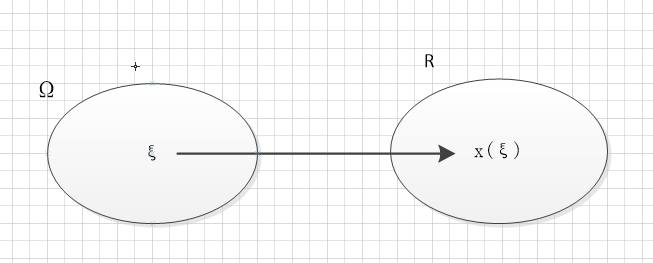
\includegraphics[scale=0.3]{xi_map}
\end{figure}
\begin{itemize}
\item 可用随机变量$x(\xi)$描述事件。\\
例掷一颗骰子(色子),设出现的点数记为随机事件A,表示``掷出的点数大于3''的事件A,可表示为``$x(\xi)>3$''。反过来,A的一个变化范围表示一个随机事件:``$2<x(\xi)<5$''表示事件``掷出的点数大于2且小于5''。
\item 随机变量随着试验的结果而取不同的值,在试验之前不能确切知道它取什么值,但是随机变量的取值有一定的统计规律性---概率分布。
\end{itemize}
\end{frame}

\begin{frame}{离散型随机变量}
\begin{definition}[离散型随机变量]
	定义在样本空间$\Omega$上,取值于实数域$\mathbb{R}$,且只取有限个或可列个值的变量$x=x(\xi)$, 称作是\textbf{一维(实值)离散型随机变量}。\\
\end{definition}
\begin{block}{``可列个''值}
	所谓``可列个''值,是指这个变量所取的值可依某种次序一一列举,排成一列。例如自然数全体就是可列的。
\end{block}
\end{frame}

\begin{frame}
\begin{example}
	设$\Omega=$\{某公司2018年对某险种售出的保单\}, 对$\xi\in\Omega$, 令
	\[x(\xi)=\xi\text{在一年中的索赔次数}\]
	则$x(\xi)$是$\Omega$上的一个一维离散型随机变量, $x(\xi)$的可能取值范围为$\{0,1,2,\dots\}$。 在试验(即签定某一份保单)之前,并不能断定$x$会取哪一个值,但是我们可以知道$(x=0),(x=1),\dots$这些事件发生的概率(也就是在总体中所占的比例)$P[x(\xi)]$。\\
	离散型随机变量$x(\xi)$的可能取值为$a_i(i=1,2,\dots)$, 相应的取值$a_i$的概率$P(x(\xi)=a_i)=p_i$,写成如下表格形式, 制表称为随机变量$x(\xi)$的\textbf{分布列},也称为\textbf{分布列},简称\textbf{分布}。\\
	\centering
	\begin{tabular}{|c|c|c|c|}
		\hline 
		$x(\xi)$ & $a_1$ & $a_2$ & $\cdots$\\ 
		\hline 
		$P[x(\xi)]$ & $P[x(\xi)=a_1]$ & $P[x(\xi)=a_2]$ & $\cdots$\\ 
		\hline 
	\end{tabular} 
\end{example}
\end{frame}

\begin{frame}
\begin{example}
	在$n=5$的伯努利试验中,设事件A在一次试验中出现的概率为$p$,即$P(A)=p,P(\overline{A}=q=1-p)$, 令
	\[x(\xi)=\text{5次试验中事件A出现的次数}\]
	则
	\[P[x(\xi)=k]=C_5^kp^kq^{5-k} \]
	\centering
		\begin{tabular}{|c|c|c|c|c|c|c|}
		\hline 
		$x(\xi)$ & 0 & 1 & 2 & 3 & 4 & 5\\ 
		\hline 
		$P[x(\xi)]$ & $q^5$ & $5pq^4$ & $10p^2q^3$ & $10p^3q^2$ & $5p^4q$ & $p^5$\\	\hline 
	\end{tabular} 	
\end{example}
\end{frame}


\begin{frame}{离散型随机变量$\xi$的分布列的性质}
\begin{block}{离散型随机变量$\xi$的分布列}
	\begin{tabular}{|c|c|c|c|}
		\hline 
		$\xi$ & 0 & 1 & $\cdots$\\ 
		\hline 
		$P(\xi)$ & $p_1$ & $p_2$ & $\cdots$\\ 
		\hline 
	\end{tabular} 
\end{block}

由概率的性质可知,任一离散型随机变量的分布$\{p_i\}$都有下述两个性质:
\begin{enumerate}
	\item $p_i\ge 0,i=1,2,...$
	\item $\sum\limits_{i=1}^{+\infty}{p_i}=1$.
\end{enumerate}
反过来,任意一个具有以上两个性质的数列$\{p_i\}$,都有资格作为某一个随机变量的分布列。
\end{frame}

\begin{frame}
分布列不仅明确地给出了$(\xi=a_i)$的概率,而且对于任意一个的实数a,b,事件$(a\le\xi\le b)$发生的概率均可由分布列算出,因为
\[(a\le\xi\le b)=\bigcup_{a\le\xi\le b}(\xi=a_i)\]
于是由概率的可列加性有
\[P(a\le\xi\le b)=\sum_{i\in I_{a,b}}P(\xi=a_i)=\sum_{i\in I_{a,b}}p_i\]
其中$I_{a,b}=\{i:a\le a_i\le b\}$,即使对$\mathbb{R}$中更复杂可列的集合$B$,也有
\[P(\xi\in B)=\sum_{i\in I(B)}P(\xi=a_i)=\sum_{i\in I(B)}p_i\]
其中$I(B)=\{i:a_i\in B\}$\\
由知此可,$x(\xi)$取各种值的概率都可以由它的分布列通过计算而得到。
\begin{block}{}
	分布列全面地描述了离散型随机变量$x(\xi)$的统计规律。
\end{block}
\end{frame}

\section{几种重要的离散型随机变量的分布}

\begin{frame}
\begin{block}{二项分布}
	若试验E只有两种可能结果,一种是事件A出现,另一种是事件$\overline{A}$出现,$P(A)=p$, 称试验E为伯努利(Bernoulli)试验。现将试验E独立重复n次,若用$\xi$表示事件A出现的次数,在这n重伯努利试验中,事件A恰好出现k次的概率为
	\[P\{\xi=k\}=C_{n}^{k}p^{k}(1-p)^{n-k},\qquad k=0,1,2,\dots,n\]
\end{block}
\begin{definition}[二项分布]
	若$\xi$的概率分布是
	\[P\{\xi=k\}=C_{n}^{k}p^{k}(1-p)^{n-k},\qquad k=0,1,2,\dots,n\]
	则称$\xi$服从参数为n,p的二项分布,记作$\xi\sim B(n,p)$。
\end{definition}
\begin{block}{Notes}
	n次伯努利试验是相互独立的事件,就是试验的结果是相互独立的。
\end{block}
\end{frame}

\begin{frame}
一个伯努利试验的结果(样本点)为:
\[\xi=(\xi_1,\xi_2,\dots,\xi_n)\]
其中的$\xi_i(1\le i\le n)$或者是$A$或者是$\overline{A}$,因而这样的$\xi$共有$2^n$个,它们的全体就是这个伯努利试验的样本空间$\Omega$,对于$\xi=(\xi_1,\xi_2,\dots,\xi_n)\in\Omega$, 如果$\xi_i(1\le \xi\le n)$中有$k$个为$A$, 则必有$n-k$个为$\overline{A}$,于是由独立性即得
\[P(\xi)=p^k(1-p)^{n-k}\]
如果要求``$n$重伯努利试验中事件$A$出现$k$次''这一事件的概率,为此记
\[B_k=\{\text{$n$重伯努利试验中事件$A$出现$k$次}\}\]
由概率的有限可加性记得
\[P(B_k)=\sum_{\xi\in B_k}P(\xi)\]
对于$\xi\in B_k$,已知$P(\xi)=p^k(1-p)^{n-k}$, 而$B_k$中这样的$\xi$共有$C_{n}^{k}$个,所以
\[P(B_k)=C_n^k p^k(1-p)^{n-k},\qquad 0\le k\le n\]
\end{frame}

\begin{frame}
\begin{example}
   抛掷一枚硬币,出现正面的概率$p=\frac{1}{2}$,``抛掷n枚相同的硬币,恰好出现k个正面"这一事件的概率, 就是n重伯努利试验。\\
   \[P(\xi=k)=C_n^kp^k(1-p)^{n-k}=C_n^k(\frac{1}{2})^n\]
\end{example}
\begin{example}
一批产品的废品率为0.03,进行20次独立重复抽样,求出现废品的频率为0.1的概率。\\
令$\xi$表示在这20次独立重复抽样中出现的废品数,则$\xi\sim B(20,0.03)$。于是
\[P\{\frac{\xi}{20}=0.1\}=P\{\xi=2\}=C_{20}^{2}0.03^{2}(0.97)^{18}\approx 0.0988\]
\end{example}
\end{frame}

\begin{frame}
金工车间由10台同类型的机床,每台机床配备的电动机功率为10千瓦,已知每台机床工作时,平均每小时实际开动12分钟,且开动与否是相互独立的。现因当地电力供应紧张,供电部门只提供50千瓦的电力给这10台机床。问这10台机床能够正常工作的概率为多大?\\
解 50千瓦电力可同时供给5台机床工作(开动),因而10台机床中同时开动的台数不超过5台时都可以正常工作。每台机床正常工作的概率$p=\frac{12}{60}=\frac{1}{5}$。设10台机床中正常工作的机床台数为$\xi$,则
\[P(\xi=k)=C_n^kp^k(1-p)^{n-k}=C_{10}^k(\frac{1}{5})^k(\frac{4}{5})^{10-k},\quad 0\le k\le 10 \]
于是同时正常工作着的机床台数不超过5台的概率为
\begin{align*}
P(\xi\le 5) &= \sum_{k=0}^{5}P(\xi=k)\\
&=\sum_{k=0}^{5}C_{10}^k(\frac{1}{5})^k(\frac{4}{5})^{10-k}\approx 0.994
\end{align*}
\end{frame}

\begin{frame}
某大学的校乒乓球队与数学系乒乓球队举行对抗赛。校队的实力比系队强,当一个校队的运动员与一个系队的运动员比赛时,校队运动员获胜概率为0.6。 校、系双方对抗赛有以下三种方案:\\
(1) 双方各出3人,比三局; (2) 双方各出5人,比五局; (3) 双方各出7人,比七局。\\
三种方案中均以比赛中得胜人数多得一方为胜利。问: 对系队来说,哪一种方案有利?
\begin{block}{}
	设系队得胜人数为$\xi$, 则在上述三种方案中,系队胜利的概率为:
	\begin{align*}
	(1) P(\xi\ge 2) &=\sum_{k=2}^{3}C_3^k(0.4)^k(0.6)^{3-k}\approx 0.352\\
    (2) P(\xi\ge 3) &=\sum_{k=3}^{5}C_5^k(0.4)^k(0.6)^{5-k}\approx 0.317\\
    (3) P(\xi\ge 4) &=\sum_{k=4}^{7}C_7^k(0.4)^k(0.6)^{7-k}\approx 0.290\\
	\end{align*}
\end{block}
\end{frame}

\begin{frame}{随机变量的分布函数}
\begin{definition}
	设$\xi$是随机变量, 对$\forall x\in\mathbb{R}$, 称函数
	\[F(x)=P\{x(\xi)\le x\}\]
	为随机变量$x(\xi)$的(累积)分布函数[(cumulative) distribution function]。
\end{definition}
\begin{block}{分布函数性质}
\begin{enumerate}
	\item 单调不减性: 对$\forall x_1<x_2$, 恒有$F(x_1)\le F(x_2)$
	\item 规范性: $F(-\infty)=\lim\limits_{x\to -\infty}F(x)=0$, $F(+\infty)=\lim\limits_{x\to +\infty}F(x)=1$
	\item 右连续性: 对$\forall x_0$, 恒有$F(x_0+0)=\lim\limits_{x\to x_0^+}F(x)=F(x_0)$
\end{enumerate}
\end{block}
\end{frame}

\begin{frame}{随机变量的概率密度函数}
\begin{definition}
	设连续随机变量$x(\xi)$的一维累积分布函数为$F(x)$, 如果$F(x)$对$x$的一阶导数存在,则有
	\[p(x)\mathop{=}^{def}\frac{dF(x)}{dx}\]
	式中, $p(x)$称为随机变量$x(\xi)$的一维概率密度函数, 简称概率密度函数(probability density function,p.d.f)
\end{definition}
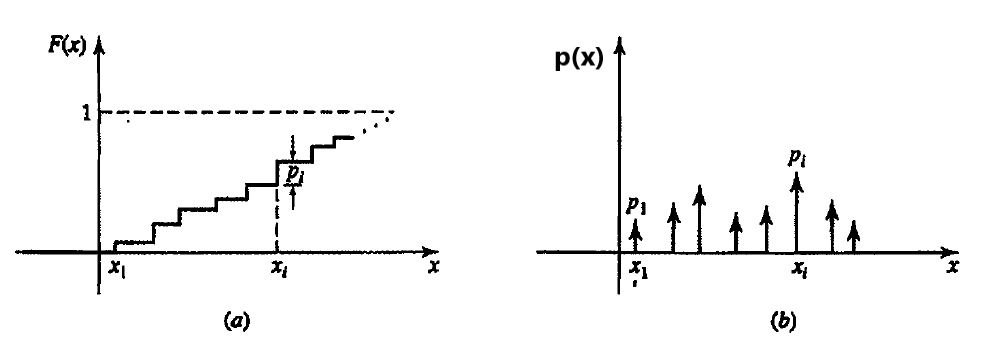
\includegraphics[scale=0.4]{pi}
\end{frame}

\begin{frame}[shrink]
\frametitle{随机变量概率密度函数性质}
\begin{enumerate}
	\item 根据随机变量$x(\xi)$的$p(x)$与$F(x)$的关系, 有
	\[F(x)=\int_{-\infty}^{x}p(u)du\]
	\item 对所有$x$, p(x)是非负函数,即
	\[p(x)\ge 0,\quad -\infty<x<+\infty \]
	\item $p(x)$对$x$的全域积分结果等于1, 一般表示为
	\[\int_{-\infty}^{\infty}p(x)dx=1\]
	\item 随机变量$x(\xi)$落在区间$[x_1,x_2]$内的概率为
	\[P\{x_1\le x(\xi)\le x_2\}=F(x_2)-F(x_1)=\int_{x_1}^{x_2}p(x)dx\]
\end{enumerate}
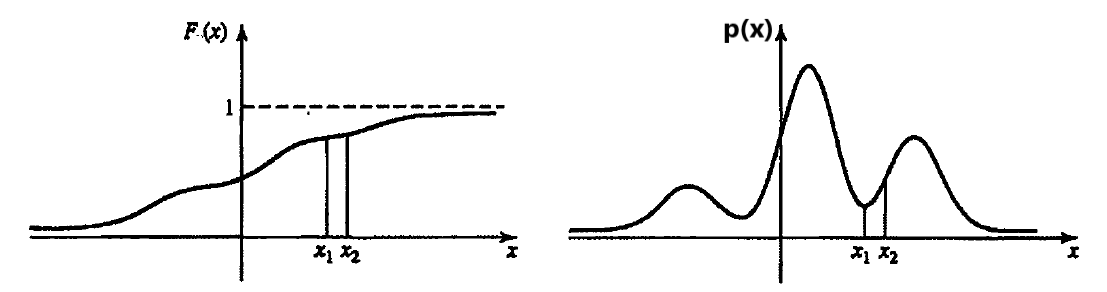
\includegraphics[scale=0.3]{Fx-px2}
\end{frame}

\begin{frame}[shrink]
抛掷一枚硬币: 样本空间: $\Omega=\{h,t\}$, $h$表示正面, $t$表示反面。正面的概率$p$, 反面的概率$q$. 定义随机变量$x(\xi),\xi\in \Omega$满足:
	\[x(\xi=h)=x(h)=1\qquad x(\xi=t)=x(t)=0,\]
	求$F(x)$,其中: $-\infty<x<\infty$.\\
	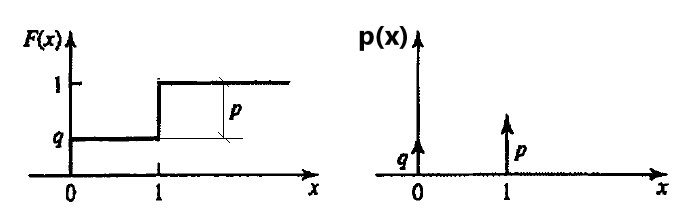
\includegraphics[scale=0.4]{coin-tossing}\\
	如果$x\ge 1$, 则$x(h)=1\le x$, 且$x(t)=0\le x$, 有
	\[F(x)=P\{x(\xi)\le x \}=P\{h,t\}=1\qquad x\ge 1 \] 
    如果$0\le x<1$, 则$x(h)=1> x$, 且$x(t)=0\le x$, 有
    \[F(x)=P\{x(\xi)\le x \}=P\{t\}=q \qquad 0\le x<1 \] 
    如果$x<0$, 则$x(h)=1> x$, 且$x(t)=0> x$, 有
    \[F(x)=P\{x(\xi)\le x \}=P\{\emptyset\}=0 \qquad x<0 \] 
\end{frame}

\begin{frame}[shrink]
事件A, 试验的样本空间: $\Omega=\{A,\overline{A},\emptyset \}$. 定义随机变量$x(\xi)$,
满足:
\begin{align*}
	x(\xi)=1, &\quad \xi\in A\\
	x(\xi)=0, &\quad \xi\in\overline{A}
\end{align*}
$P(A)=p,P(\overline{A})=q=1-p$
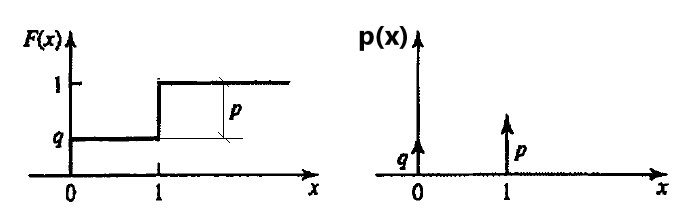
\includegraphics[scale=0.4]{coin-tossing}\\
如果$x\ge 1$, 则$\{x(\xi)\le x\}=\{\Omega \}$, 有
\[F(x)=P\{x(\xi)\le x \}=P\{\Omega \}=1\qquad x\ge 1 \] 
如果$0\le x<1$, 则$\{x(\xi)\le x\}=\{\overline{A}\}$, 有
\[F(x)=P\{x(\xi)\le x \}=P\{\overline{A}\}=q \qquad 0\le x<1 \] 
如果$x<0$, 则$\{x(\xi)\le x\}=\{\emptyset\}$, 有
\[F(x)=P\{x(\xi)\le x \}=P\{\emptyset\}=0 \qquad x<0 \] 
\end{frame}

\begin{frame}[shrink]
抛掷两枚硬币: 随机变量$x(\xi)$表示正面数目。求$F(x)$.\\
样本空间: $\Omega=\{HH,HT,TH,TT\}$, $H$表示正面, $T$表示反面。\\
随机变量$x(\xi)$: $x(HH)=2,\quad x(HT)=1, \quad x(TH)=1, \quad x(TT)=0$
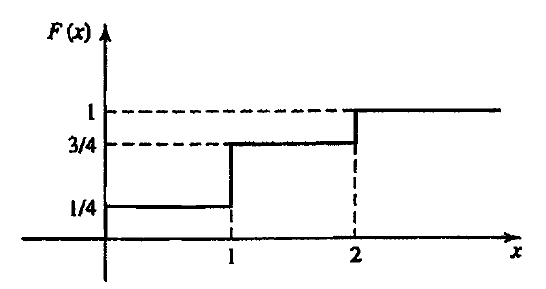
\includegraphics[scale=0.3]{coin-tossing2}\\
如果$x\ge 2$, $\{x(\xi)\le x\}=\Omega \Rightarrow F(x)=1$ \\
如果$1\le x<2$, $\{x(\xi)\le x\}=\{TT,HT,TH\} \Rightarrow F(x)=P\{TT\}+P\{HT\}+P\{TH\}=\frac{3}{4}$ \\
如果$0\le x<1$, $\{x(\xi)\le x\}=\{TT\} \Rightarrow F(x)=P\{TT\}=P(T)P(T)=\frac{3}{4}$ \\
如果$x<0$, $\{x(\xi)\le x \}=\emptyset \Rightarrow F(x)=0$ \\
当$x=1$, $P\{x(\xi)=1\}=F(1)-F(1^{-})=3/4-1/4=1/2$
\end{frame}

\begin{frame}[shrink]
掷一枚骰子: 样本空间: $\Omega=\{f_1,f_2,f_3,f_4,f_5,f_6\}$。定义随机变量$x(\xi),\xi\in \Omega$满足:$x(f_i)=10i$
求$F(x)$,其中: $-\infty<x<\infty$.\\
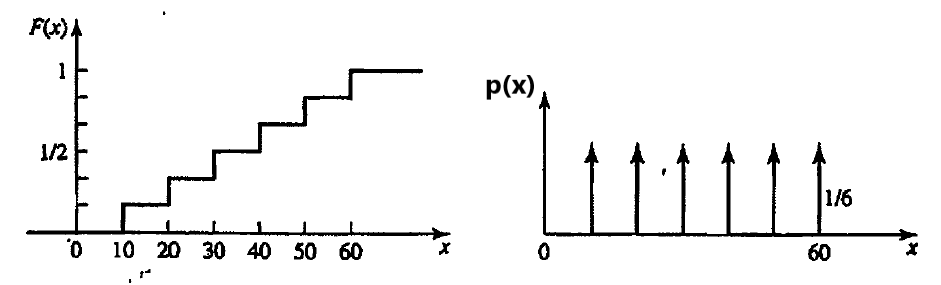
\includegraphics[scale=0.4]{die}
\begin{align*}
F(100)&=P\{x(\xi)\le 100 \}=P(\Omega)=1\\
F(35)&=P\{x(\xi)\le 35 \}=P\{f_1,f_2,f_3 \}=\frac{3}{6} \\
F(30.01)&=P\{x(\xi)\le 30.01 \}=P\{f_1,f_2,f_3 \}=\frac{3}{6} \\
F(30)&=P\{x(\xi)\le 30 \}=P\{f_1,f_2,f_3 \}=\frac{3}{6} \\
F(29.9)&=P\{x(\xi)\le 35 \}=P\{f_1,f_2 \}=\frac{2}{6} \\
\end{align*}
\end{frame}

\begin{frame}
\begin{columns}
	\column{0.5\textwidth}
	均匀分布随机变量$x(t)=t,0<t<T$\\
	$P\{t_1\le t\le t_2\}=\frac{t_2-t_1}{T},0<t_1<t_2<T$\\
	如果$x> T$, 有
	\[F(x)=P\{x(t)\le x \}=P\{0\le t\le T \}=P(\Omega)= 1\qquad x> 1 \] 
	如果$0\le x\le T$, 有
	\[F(x)=P\{x(t)\le x \}=P\{0\le t\le x\}=\frac{x}{T} \qquad 0\le x\le 1 \] 
	如果$x<0$, 有
	\[F(x)=P\{x(t)\le x \}=P\{\emptyset\}=0 \qquad x<0 \] 
	\column{0.4\textwidth}
	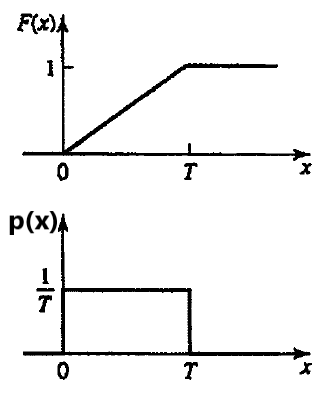
\includegraphics[scale=0.4]{xt}
\end{columns}
\end{frame}

\begin{frame}
\begin{columns}
	\column{0.5\textwidth}
	定义随机变量$x(\xi)$, 满足$\forall xi\in\Omega, x(\xi)=a$\\
	如果$x\ge a$, 则,$\forall \xi\in\Omega, x{\xi}=a\le x$,有
	\[F(x)=P\{x(\xi)\le x \}=P(\Omega)= 1\qquad x\ge a \] 
	如果$x<a$, 有
	\[F(x)=P\{x(t)\le x \}=P\{\emptyset\}=0 \qquad x<a \] 
	\column{0.4\textwidth}
	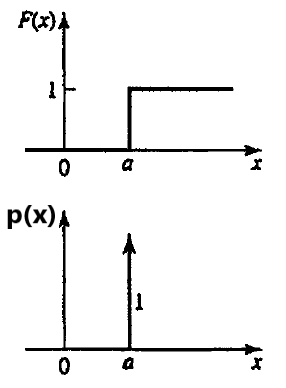
\includegraphics[scale=0.4]{a}
\end{columns}
\end{frame}

\begin{frame}[shrink]
非负实数集合$\{p_i\}$,$\forall i, i=1,2,\dots,\infty$满足, 
\begin{enumerate}
	\item $P\{x(\xi)=x_i\}=p_i$
	\item $\sum\limits_{i=1}^{\infty}p_i=1$
\end{enumerate}
求$F(x)$,其中: $-\infty<x<\infty$.\\
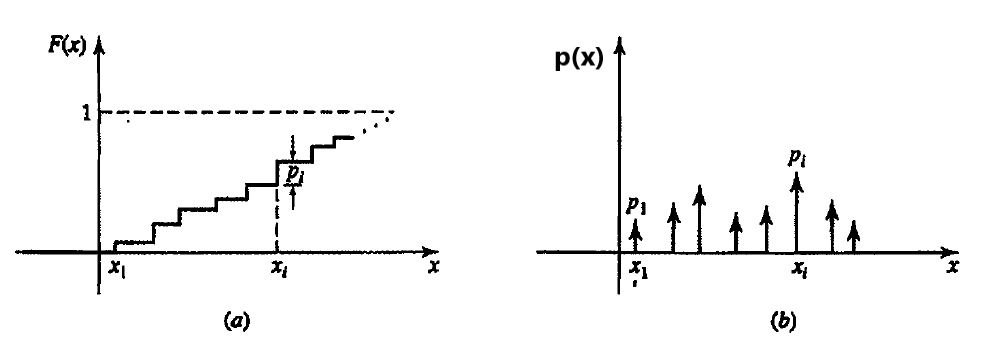
\includegraphics[scale=0.4]{pi}\\
对于$x_i\le x<x_{i+1}$, 我们有$\{x(\xi)\le x \}=\bigcup\limits_{x_k\le x}\{x(\xi)=x_k\}=\bigcup\limits_{k=1}^{i}\{x(\xi)=x_k\}$, 因此
\begin{align*}
F(x)=P\{x(\xi)\le x\}=\sum\limits_{k=1}^{i}p_k \qquad x_i\le x<x_{i+1}
\end{align*}
\end{frame}

\begin{frame}{离散型随机变量$x(\xi)$的$p(x)$}
\[P\{x(\xi)=x_i\}=F(x_j)-F(x_i^{-})=p_i\]
\[p(x)=\sum\limits_{i}p_i\delta(x-x_i) \]
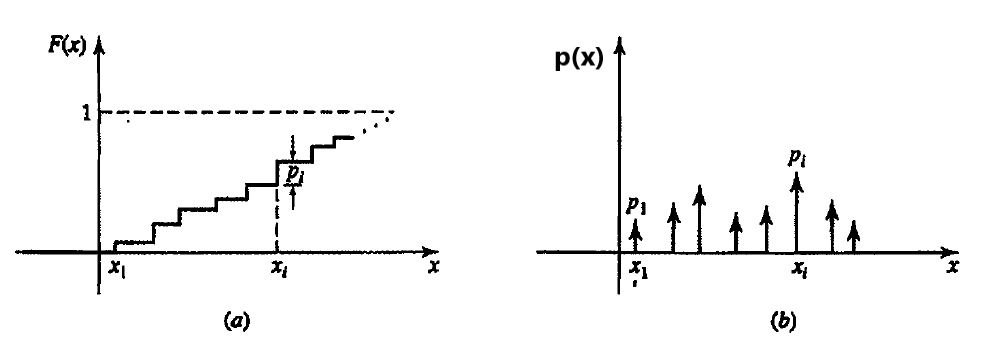
\includegraphics[scale=0.3]{pi}\\
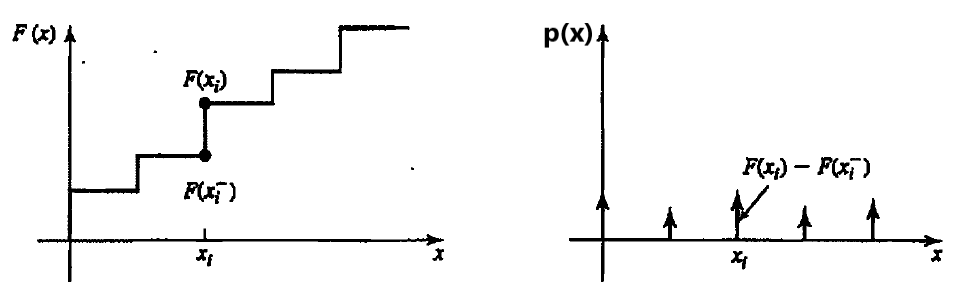
\includegraphics[scale=0.3]{Fx-px}
\end{frame}

\begin{frame}
\begin{example}
	某产品40件,其中次品3件,现从中任取3件。(1) 求取出的3件产品中所含次品数$\xi$的分布列; (2) 求取出的产品中至少有一件次品的概率; (3) 求$x(\xi)$的分布函数$F(x)$。
	\begin{block}{}
		(1) \begin{tabular}{ll}
			$P\{\xi=0\}=\frac{C_{37}^{3}}{C_{40}^{3}}=0.7865$ & $P\{\xi=1\}=\frac{C_{3}^{1}C_{37}^{2}}{C_{40}^{3}}=0.2022$ \\ 
			$P\{\xi=2\}=\frac{C_{3}^{2}C_{37}^{1}}{C_{40}^{3}}=0.0112$ & $P\{\xi=3\}=\frac{C_{3}^{3}}{C_{40}^{3}}=0.0001$ \\ 
		\end{tabular}\\ 
	   (2) $P\{\xi\ge 1\}=1-P\{\xi=0\}=1-0.7865=0.2135$\\
	   (3) 由分布函数定义得:
	   $F(x)=P\{x(\xi)\le x\} =
	   \begin{cases}
	   	0,      & x<0 \\
	   	0.7865, & 0\le x<1 \\
	   	0.9887, & 1\le x<2 \\
	   	0.9999, & 2\le x<3 \\
	   	1,      & x\ge 3
	   \end{cases} $
	\end{block}
\end{example}
\end{frame}

\begin{frame}
\begin{block}{解:}
		(1) \begin{tabular}{ll}
			$P\{\xi=0\}=\frac{C_{37}^{3}}{C_{40}^{3}}=0.7865$ & $P\{\xi=1\}=\frac{C_{3}^{1}C_{37}^{2}}{C_{40}^{3}}=0.2022$ \\ 
			$P\{\xi=2\}=\frac{C_{3}^{2}C_{37}^{1}}{C_{40}^{3}}=0.0112$ & $P\{\xi=3\}=\frac{C_{3}^{3}}{C_{40}^{3}}=0.0001$ \\ 
		\end{tabular}\\ 
		(2) $P\{\xi\ge 1\}=1-P\{\xi=0\}=1-0.7865=0.2135$\\
		(3) 由分布函数定义得:
		$F(x)=P\{x(\xi)\le x\} =
		\begin{cases}
		0,      & x<0 \\
		0.7865, & 0\le x<1 \\
		0.9887, & 1\le x<2 \\
		0.9999, & 2\le x<3 \\
		1,      & x\ge 3
		\end{cases} $
		\begin{columns}%0.6 0.4表示相对比例
			\column{0.4\textwidth}%<1->
			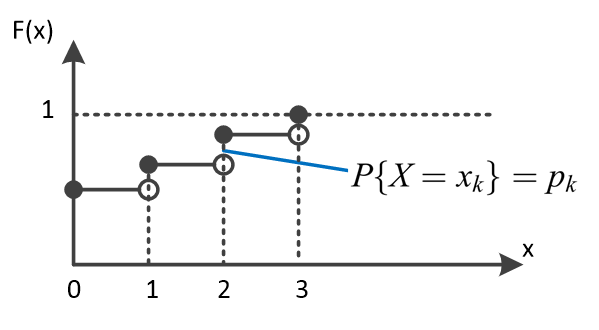
\includegraphics[scale=0.5]{fx}
			\column{0.6\textwidth}%<1->
			由$F(x)$的图示看到, $F(X)$是一个阶梯状的右连续函数($F(x+0)=F(x)$),在$x=k$处有跳跃,跃度为$\xi$在$x=k$处的概率。\\
            $F(k)-F(k-0)=P(\xi=k), k=0,1,2,3,\dots$			
	    \end{columns}
\end{block}
\end{frame}

\begin{frame}
\begin{columns}
	\column{0.4\textwidth}
	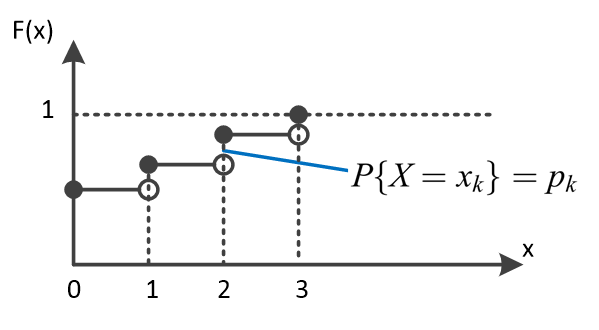
\includegraphics[scale=0.5]{fx}
	\column{0.6\textwidth}
	由随机变量$x(\xi)$的分布函数$F(x)$, 可以计算
	\begin{block}{}
		\begin{align*}
		P(x(\xi)\le x) &= F(x)\\
		P(x(\xi) = x) &= F(x)-F(x-0) \\
		P(x(\xi) < x) &= F(x-0) \\
		P(x(\xi) > x) &= 1- F(x) \\
		P(x(\xi) \ge x) &= 1-F(x-0)
		\end{align*}
		进一步,形如$\{x_1\le x(\xi)\le x_2\},\{x_1< x(\xi)< x_2\},\{x_1< x(\xi)\le x_2\}, \{x_1\le x(\xi)< x_2\}$等一些事件及它们经过有限次或可列次并、交、差运算以后的概率,都可以由$F(x)$算出来。
	\end{block}
 \end{columns}
\begin{block}{}
	$F(x)$全面地描述了随机变量$x(\xi)$地统计规律。既然分布函数能够描述一般的随机变量的统计规律,因而分布函数这个概念比分布列更重要。只不过对离散型随机变量来说,分布列比较方便。
\end{block}
\end{frame}

\begin{frame}{离散性随机变量的分布函数与分布列之间的关系}
\[F(x)=P(x(\xi)\le x)= \sum_{a_i\le x}P(x(\xi)=a_i)\]
\begin{columns}
	\column{0.4\textwidth}
	\begin{block}{离散型随机变量$\xi$的分布列}
		\begin{tabular}{|c|c|c|c|}
			\hline 
			$x(\xi)$    & $a_1$ & $a_2$ & $\cdots$\\ 
			\hline 
			$P(x(\xi))$ & $p_1$ & $p_2$ & $\cdots$\\ 
			\hline 
		\end{tabular} 
	\end{block}
	\column{0.4\textwidth}
	\begin{block}{离散型随机变量$\xi$的分布函数}
		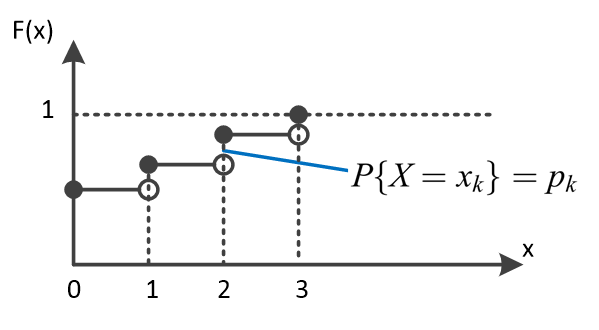
\includegraphics[scale=0.5]{fx}
	\end{block}
\end{columns}
\end{frame}

\begin{frame}
\begin{example}
	若$\xi$只取一个值$a$, 即有$P(\xi=a)=1$, 求$\xi$的分布函数$F(x)$.
\end{example}
\begin{block}{解}
	\[
	 F(x)=P(\xi\le x)= 
	 \begin{cases}
	 1, &x\ge a\\
	 0, &x<a
	 \end{cases}
	\]
	\begin{columns}
		\column{0.4\textwidth}	
		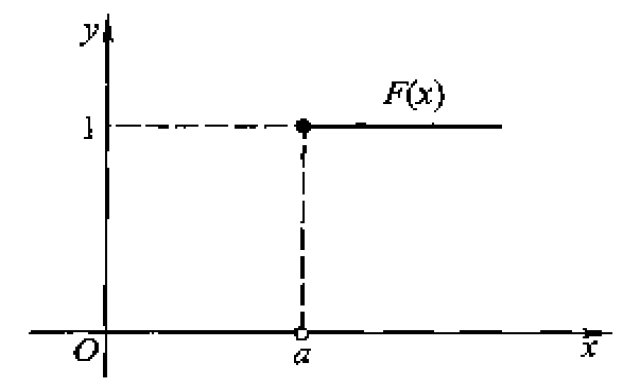
\includegraphics[scale=0.3]{fx1}
		\column{0.4\textwidth}
		如图所示,$F(x)$是一个右连续的、阶梯状的函数,在$x=a$处有一个跳跃,其跃度为
		\[1=P(\xi=a)\]
	\end{columns}
\end{block}
\end{frame}

\begin{frame}
\begin{example}
	等可能地在$[a,b]$上投点,所投的点落在$[a,b]$中的任一子区间$B=[c,d]$中的概率与$B$的长度$l_B$成正比,而与$B$在$[a,b]$中的位置无关。如果记``点落入$B$中"这一事件为$B$,则上述等可能性意味着
	\[P(B)=\frac{l_B}{b-a}=\frac{d-c}{b-a}\]
	如果投在$[a,b]$中的点的坐标为$\xi(a\le\xi\b)$令
	\[x(\xi)=\xi\qquad (a\le\xi\b)\]
	这样就得到一个随机变量$x(\xi)$,它的取值充满了整个区间$[a,b]$.
	对于任意一点$\xi_0$的概率为: 
	\[P(x(\xi)=\xi_0)=P(\xi=\xi_0)=\frac{l_{\xi_0}}{b-a}=0\]
	由于单点集的长度为零。
	因此用``分布列"研究随机变量$x(\xi)$的统计规律是行不通的。引入分布函数的概念。
\end{example}
\end{frame}

\begin{frame}
点落落入$B=[c,d]$区间的概率与$B$的长度$l_B$成正比,设$B=[c,d]\subset [a,b]$,就有
	\[P(c\le d)=P(\text{点落入$B$中})=P(B)=\frac{d-c}{b-a} \]
	因为$P(\xi =c)=0$,所以
	\[a\]
\end{frame}

%%%%%%%%%%%%%%%%%%%%%%%%%%%%%%%%%%%%%%%%%%%%%%%%%%%%%

注释的内容
%%%%%%%%\iffalse  %注释开始

\begin{frame}
n重伯努利试验k次成功的概率(二项分布):
\[P\{\xi=k\}=C_{n}^{k}p^{k}(1-p)^{n-k},\qquad k=0,1,2,\dots,n\]
特例:令二项分布的$n=1$, $k$只能取0或1,描述事件A发生的概率。

\begin{definition}[0--1分布]
	若$x(\xi)$的概率分布是\\
	\begin{center}
	\begin{tabular}{|c|c|c|}
		\hline 
		$\xi$ & 0 & 1\\ 
		\hline 
		$P(\xi)$ & $1-p$ & $p$\\ 
		\hline 
	\end{tabular} \\
	\end{center}
	则称$x(\xi)$服从参数$p$的0--1分布。
\end{definition}

\end{frame}

\begin{frame}
\begin{example}
	抛掷一枚硬币, $p=1-p=\frac{1}{2}$。\\
	\begin{tabular}{|c|c|c|}
		\hline 
		$\xi$ & 0(正面朝上) & 1(正面朝下)\\ 
		\hline 
		$P(\xi)$ & $0.5$ & $0.5$\\ 
		\hline 
	\end{tabular} 
\end{example}

\begin{example}
	一批产品的废品率为5\%, 从中任取一个进行检查, 若令$\xi$表示取得废品的数量,写出$\xi$的概率分布。\\
	\begin{tabular}{|c|c|c|}
		\hline 
		$\xi$ & 0 & 1\\ 
		\hline 
		$P(\xi)$ & $0.95$ & $0.05$\\ 
		\hline 
	\end{tabular} 
\end{example}
\end{frame}

\begin{frame}
在一个努利试验中,每次试验成功的概率为$p$,失败的概率为$1-p$,设试验进行到第k次才成功,试验结束。
第k次才成功,表明k-1次是的失败的,概率为$(1-p)^{k-1}$, 有独立性即得总的概率为$(1-p)^{k-1}p$。

\begin{definition}[几何分布]
	若$x(\xi)$的概率分布是
	\[P(\xi=k)=(1-p)^{k-1}p,\qquad (0<p<1,k=1,2,\dots)\]
	则称$x(\xi)$服从参数为$p$的几何分布,记作$\xi\sim G(p)$
\end{definition}
\end{frame}

\begin{frame}
\begin{example}
	社会上定期发行某种奖券,每券一元,中奖率为$p$,某人每次购买1张奖券, 如果没有中奖,下次继续购买一张,直到中奖为止。求该人购买奖券次数$\xi$的概率分布。\\
	令$A_k=$\{第$k$次购买的奖券中奖\}, $k=1,2,3,...$, \\
	则$P(A_k)=p,\quad P(\overline{A_k})=1-p$, \\
	由于$A_1,A_2,A_3,\dots$相互独立,于是:
	\begin{align*}
	P(\xi=1)&=P(A_1)=p\\
	P(\xi=2)&=P(\overline{A_1}A_1)=P(\overline{A_1})P(A_2)=(1-p)p\\
	P(\xi=3)&=P(\overline{A_1}\overline{A_2}A_3)=P(\overline{A_1})P(\overline{A_2})P(A_3)=(1-p)^{2}p\\
	\cdots\\
	P(\xi=k)&=P(\overline{A_1}\overline{A_2}\cdots\overline{A_{k-1}}A_k)=P(\overline{A_1})P(\overline{A_2})\cdots P(\overline{A_{k-1}})P(A_k)=(1-p)^{k-1}p
	\end{align*}
	$\implies \xi\sim G(p)$
\end{example}
\end{frame}

\begin{frame}
\begin{example}
	某射手命中率为$p,(0<p<1)$,现有五发子弹。射击一发,如果命中,即停止射击,否则再射击一次,依次类推,如用$\eta$表示他射击所用去的子弹数,求$\eta$的分布。\\
	当$(\eta=k),1\le k\le 4$时表示前$(k-1)$次射击均未命中。第$k$次才首次命中,依题意,每次射击是相互独立的。故$P(\eta=k| 1\le k\le 4)=(1-p)^{k-1}p$。而$(\eta=5)$时表示前4次射击均未命中,第5次射击后不管是否命中均要停止。故$P(\eta=k|k=5)=(1-p)^{k-1}p$。\\
	\begin{tabular}{|c|c|c|c|c|c|}
		\hline 
		$\eta$ & 1 & 2 & 3 & 4 & 5\\ 
		\hline 
		$P(\eta)$ & $p$ & $p(1-p)$ & $p(1-p)^2$ & $p(1-p)^3$  & $(1-p)^4$ \\ 
		\hline 
	\end{tabular} 
\end{example}
\end{frame}

\begin{frame}
\begin{example}
	设随机相位正弦信号$s(t; \theta)=a\cos(\omega_0 t+\theta)$, 其中振幅$a$和$\omega_0$为常数, 相位$\theta$是一随机变量,它服从$[-\pi,\pi]$上的均匀分布。
	\begin{enumerate}
		\item 求该过程的均值$E[s(t; \theta)]$和自相关函数$E[s(t_j; \theta)s(t_k; \theta)]$。
		\item 写出$s(t;\theta)$的样本函数。
		\item 求$s(t;\theta)$的概率密度函数。
	\end{enumerate}
\end{example}
\end{frame}

\begin{frame}
解:
\begin{enumerate}
\item 因为相位$\theta$服从$[-\pi,\pi]$上的均匀分布,所以,
$$p(\theta)=\begin{cases}
\frac{1}{2\pi}, & -\pi\le\theta\le\pi\\
0, &\text{其它}
\end{cases} $$ 
该随机过程的均值为:
\begin{align*}
\mu_{\theta}(t)&=E[s(t; \theta)]=E[a\cos(\omega_0t+\theta)]\\
&=\int_{-\infty}^{\infty}a\cos(\omega_0t+\theta)p(\theta)d\theta\\
&=\int_{-\pi}^{\pi}a\cos(\omega_0t+\theta)\frac{1}{2\pi}d\theta\\
&=\frac{a}{2\pi}\int_{-\pi}^{\pi}\cos(\omega_0t+\theta)d\theta\\
&=0
\end{align*}
\end{enumerate}
\end{frame}

\begin{frame}
解(续): \footnote{$\cos A\cos B=\frac{1}{2}\cos (A+B)\cos(A-B)$}
\begin{enumerate}
\item (续) 该随机过程的自相关函数为:
\begin{align*}
r_x(t_j,t_k)&=E[s(t_j)s(t_k)]\\
&=\int_{-\infty}^{\infty}a\cos(\omega_0t_j+\theta)a\cos(\omega_0t_k+\theta)p(\theta)d\theta\\
&=\frac{a^2}{4\pi}\int_{-\pi}^{\pi}[\cos(\omega_0t_j+\omega_0t_k+2\theta)+\cos\omega_0(t_k-t_j)]d\theta\\
&=\frac{a^2}{2}\cos\omega_0\tau,\qquad(\tau=t_k-t_j)
\end{align*}
\item 当$\theta$在$[-\pi,\pi]$内任取定值时,如$\theta=0$, 则样本函数为
$$s_1(t; \theta=0)=a\cos\omega_0t$$
当$\theta=\frac{\pi}{2}$, 则样本函数为
$$s_2(t; \theta=\frac{\pi}{2})=a\cos(\omega_0t+\frac{\pi}{2})=-a\sin\omega_0t$$
\end{enumerate}
\end{frame}

\begin{frame}
解(续):
\begin{enumerate}
\setcounter{enumi}{2} %设定起始编号 
\item 求$s(t;\theta)$的概率密度函数。\\
固定时刻$t$, 则随机变量$s(t;\theta)=a\cos(\omega_0t+\theta)$是随机变量$\theta$的函数。
由分布函数的定义:
$$F_{s(t)}(y)=P\{s(t)\le y\}=P\{a\cos(\omega_0t+\theta)\le y \}$$
当$y<-a$时,$F_{x(t)}(y)=0$; 当$y\ge +a$时, $F_{x(t)}(y)=1$\\
当$-a<y\le +a$时,我们有:
\begin{align*}
F_{s(t)}(y) &=P\{x(y)\le y \}=P\{a\cos(\omega_0t+\theta)\le y \}\\
&=P(\{-\pi<\theta\le\omega_0t-\arccos\frac{y}{a} \} \cup \{\arccos\frac{y}{a}-\omega_0t<\theta\le\pi \})\\
&=\frac{1}{2\pi}\left[\int_{-\pi}^{\omega_0t-\arccos\frac{y}{a}}dx+\int_{\arccos\frac{y}{a}-\omega_0t}^{\pi}dx\right]\\
&=\frac{1}{\pi}[\omega_0t+\pi-\arccos\frac{y}{a}]
\end{align*}	
\end{enumerate}
\end{frame}

\begin{frame}
解(续):
\begin{enumerate}
\setcounter{enumi}{2} %设定起始编号 
\item (续)求$x(t;\theta)$的概率密度函数。\\
当$-a<y\le +a$时, 有: $F_{x(t)}(y)=\frac{1}{\pi}[\omega_0t+\pi-\arccos\frac{y}{a}]$\\
此时, $x(t;\theta)$的概率密度函数为:
$$p_{x(t)}(y)=F_{x(t)}^\prime(y)=\frac{1}{\pi\sqrt{a^2-y^2}} $$
最终得到$x(t;\theta)$的概率密度函数为:
$$ p(\theta;t)=
\begin{cases}
\frac{1}{\pi\sqrt{a^2-x^2}}, &-a<x\le +a \\
0,&\text{其它}
\end{cases}
$$
\end{enumerate}
\end{frame}

\begin{frame}
\begin{example}
	考察一随机过程,它在$t_0+nT_0$时刻具有宽度为b的矩形脉冲波,脉冲幅度为一等概率$(p)$,取值$\pm a$的随机变量,且$b<T_0,T_0$是在$(0,T_0)$上服从均匀分布的随机变量,并且脉冲幅度$A$与$t_0$独立, 试求该过程的自相关函数和方差。
\end{example}
解: 由给定的随机过程,我们有,均值: 
$$\mu_x(t)=E\{x(t)\}=a\times p+(-a)\times p + 0\times(1-2p)=0$$
下面求自相关函数:\\
任取$t_1,t_2$,且$t_1<t_2$,当$|t_1-t_2|>T_0$时, $t_1,t_2$位于不同的周期内,此时有:
$$r_x(t_1,t_2)=E\{x(t_1)x(t_2)\}=E\{x(t_1)\}E\{x(t_2)\}=0$$

当$|t_1-t_2|\le T_0$, 且$t_1,t_2$位于两个不同的周期内时,此时有:
$$r_x(t_1,t_2)=E\{x(t_1)x(t_2)\}=E\{x(t_1)\}E\{x(t_2)\}=0$$
\end{frame}

\begin{frame}
当$|t_1-t_2|\le T_0$, 且$t_1,t_2$位于同一周期内时,假设$\theta$为$t_1$所在的脉冲的起始时刻,只有当$t_2<\theta+b$时, $x(t_1)和x(t_2)$取到不为0的值, 此时的概率为:
$$P\{t_2<\theta+b \}=1-P\{t_2>\theta+b\}=1-\frac{1}{T_0}\int_{t_1-T_0}^{t_2-b}d\theta=\frac{b-(t_2-t_1)}{T_0}$$
由此,我们有:
$$r_x(t_1,t_2)=E\{x(t_1)\}E\{x(t_2)\}=a^2\cdot\frac{b-(t_2-t_1)}{T_0}$$
同理,当$t_1>t_2$时,我们有:
$$r_x(t_1,t_2)=E\{x(t_1)x(t_2)\}=a^2\cdot\frac{b-(t_1-t_2)}{T_0}$$
因此,最终得到自相关函数和方差:
$$r_x(\tau)=\frac{a^(b-|\tau|)}{T_0},\tau=t_2-t_1,\qquad \sigma_x^2(t)=r_x(0)=\frac{a^2b}{T_0}$$
\end{frame}

\begin{frame}{中心极限定理}
\begin{block}{高斯噪声的数学模型---中心极限定理}
	在一般条件下, $N$个相互\textbf{统计独立}的随机变量$n_i$之和$n=\sum\limits_{k=1}^{N}n_k$, 在$N\to\infty$的极限情况下,其概率密度趋于高斯分布,而不管每个变量$n_k$的具体分布如何。
\end{block}
\begin{block}{注}
	(1) 实际上,只要$N$足够大,每个分量之间也不一定完全统计独立,但不存在占统治地位的若干分量,则它们和的分布就可以近似为高斯分布。\\
	(2) 无限多的、相互独立的、各自作用有限的系统干扰分量叠加形成噪声干扰,并且服从高斯分布。
\end{block}
\end{frame}

%%%%%%%%%%\fi   %注释结束
